%documentclass[9pt]{beamer}
\documentclass[handout,9pt]{beamer}
%\usepackage{hyperref}
%\usepackage{beamerthemesplit}
\usepackage{etoolbox}
\usepackage{amsmath}
\usepackage{booktabs,multirow}
\usepackage{mathtools}
\usepackage{pgf}
\usepackage{pifont}
\usepackage{tabularx}
\usepackage{pgfplots}
\pgfplotsset{compat=1.7}
%\usepackage{xcolor}
%\usepackage{refcheck}


\makeatletter
% save the meaning of \@footnotetext
\let\BEAMER@footnotetext\@footnotetext
\makeatother


\usepackage{setspace}

\newcommand{\myfootnote}[1]{
	\renewcommand{\thefootnote}{}
	\footnotetext{\scriptsize#1}
	\renewcommand{\thefootnote}{\arabic{footnote}}
}
\setbeamertemplate{theorem begin}
{%
	\inserttheoremheadfont% \bfseries
	\inserttheoremname \inserttheoremnumber
	\ifx\inserttheoremaddition\@empty\else\ (\inserttheoremaddition)\fi%
	\inserttheorempunctuation
	\normalfont
}


\makeatletter
% restore the meaning of \@footnotetext
\let\@footnotetext\BEAMER@footnotetext
% patch the relevant command to do single spacing in footnotes
\expandafter\patchcmd\csname beamerx@\string\beamer@framefootnotetext\endcsname
{\reset@font}
{\def\baselinestretch{\setspace@singlespace}\reset@font}
{}{}
\makeatother

%\hypersetup{pdfpagemode=FullScreen}
\mode<presentation>
{
	%\usetheme{Warsaw}
	%\usetheme{Szeged}
	%\usetheme{default}
	%\usetheme{Berlin}
	%\usetheme{Berkeley}
	%\usetheme{Hannover}
	%\usetheme{Singapore}
	%\usetheme{Frankfurt}
	\usetheme{Madrid}
	%\setbeamercolor{block title}{use=structure,fg=white,bg=red!30!gray}
	%\setbeamercolor{block body}{use=structure,fg=black,bg=red!20!white}
	
	
	%\usecolortheme{wolverine}
	%\usecolortheme{crane}
	%\usecolortheme{seagull}
	%\usecolortheme{beetle}
	%\usecolortheme{seahorse}
	%\usecolortheme{rose}
	%\usecolortheme{rose}
	%\useinnertheme{circles}
	%\usecolortheme{beaver}
	%\usecolortheme[named=red]{structure}
	%\useoutertheme{smoothbars}
	%\usecolortheme[RGB={230,90,90}]{structure}
	%\usecolortheme[RGB={255,90,90}]{structure}
	%\usecolortheme[RGB={0,100,200}]{structure}%final
	%\usecolortheme[RGB={30,50,180}]{structure}
	\usecolortheme[RGB={0,160,0}]{structure}%ramesh2
	%\usecolortheme[RGB={0,228,0}]{structure}
	%\usecolortheme[RGB={220,120,200}]{structure}
	%\usefonttheme{structureitalicserif}
	%\setbeamerfont{title}{shape=\bfseries,family=\rmfamily}
	%\setbeamercolor{title}{fg=red!10!white,bg=blue!80!white}
	% or ...
	%\usebeamercolor[fg]{green}
	%\usefonttheme[large]{structuresmallcapsserif}
	\usefonttheme{serif}
	%\usefonttheme{professionalfonts}
	%\usefonttheme{structurebold}
	%\usefonttheme{structureitalicserif}
	%\usefonttheme[onlysmall]{structurebold}
	%\setbeamercovered{transparent}
	% or whatever (possibly just delete it)
	%\useoutertheme{smoothtree}
}
%\setbeamercolor{one}{bg=white, fg=red}
%\setbeamercolor{two}{bg=white,fg=blue}
%\setbeamercolor{three}{fg=blue, bg=orange}
%\setbeamercolor{four}{fg=blue, bg=yellow}
%\usebeamertemplate{logo}
\usepackage[english]{babel}
% or whatever
\usepackage{hyperref}

%\usepackage[latin1]{inputenc}
% or whatever
%\usepackage{pgfpages}
%\pgfpagelayout{resize}[a4paper, border shrink=5mm, landscape]
\usepackage{times}
\usepackage[T1]{fontenc}
\newcommand\ceil[1]{\left\lceil#1\right\rceil}
% Or whatever. Note that the encoding and the font should match. If T1
% does not look nice, try deleting the line with the fontenc.
\newtheorem{proposition}{\bf Proposition}[section]
%\newtheorem{definition}{\bf Definition}[section]
\newtheorem{remark}{\bf Remark}[section]
\newtheorem{remarks}{\bf Remarks}[section]
\newcommand\floor[1]{\lfloor#1\rfloor}
\renewcommand{\qedsymbol}{$\square$}
\numberwithin{theorem}{section}
\setbeamertemplate{theorems}[numbered]
\newcommand*{\theorembreak}{\usebeamertemplate{theorem end}\framebreak\usebeamertemplate{theorem begin}}

\makeatletter
\graphicspath{ {./images/} }
\setbeamertemplate{footline}
{
	\leavevmode%
	\hbox{%
		\begin{beamercolorbox}[wd=.5\paperwidth,ht=2.25ex,dp=1ex,center]{author in head/foot}%
			\usebeamerfont{author in head/foot}\insertshortauthor
		\end{beamercolorbox}%
		\begin{beamercolorbox}[wd=.5\paperwidth,ht=2.25ex,dp=1ex,center]{title in head/foot}%
			\usebeamerfont{title in head/foot}\insertshorttitle
		\end{beamercolorbox}%
	}%
	\vskip0pt%
}
\makeatother
\setbeamertemplate{headline}{}
\definecolor{ppp}{rgb}{0.00, 0.2, 0.6}
\newcommand{\boundellipse}[3]% center, xdim, ydim
{(#1) ellipse (#2 and #3)
}



\begin{document}
	\titlegraphic{
\includegraphics{iitbhu}}
	\title[Linear Regression]{Linear Regression - Predicting Insurance Prices}
	\subtitle{(Exploratory Project)}
	
	%\subtitle{{\color{blue}Ph.D Viva-Voce}}
	
	\author[Shrey Gupta]{\Large Mr. Shrey Gupta}
	%        {{ \Large Amit Kumar}\\
		%\vspace{0.5cm}        
		%%{(joint work with {\color{black} Dr.  Neelesh S. Upadhye and Prof. P. Vellaisamy)}}
		%}
	%%\titlegraphic{\includegraphics[width=1.4cm]{iitm.pdf}}
	%
	\institute{\small B.Tech Student\\ Mathematics and Computing\\Indian Institute of Technology (BHU)\\ Varanasi -- 221 005.}
	
	
	\date{December 6, 2021}
	
	\frame{\titlepage}
	\begin{frame}
		\frametitle{Outline}
	\tableofcontents
	\end{frame}

\section{Introduction and Motivation}

\begin{frame}
\begin{spacing}{1}
\frametitle{Introduction and Motivation}
\begin{definition}
	\textbf{What is Machine Learning ?} \pause\\
	\vspace{0.2cm}
	Machine learning is an application of artificial intelligence (AI) that provides systems the ability to automatically learn and improve from experience.\pause
\end{definition}
\begin{definition}
	\textbf{What is Linear Regression ?} \pause\\
	\vspace{0.2cm}
	Supervised learning algorithm in which we have to fit a function $f$ that maps our inputs $X$ to the corresponding function values $f(x)$.
\end{definition}
\end{spacing}
\end{frame}

\begin{frame}
	\begin{spacing}{1}
	\frametitle{Introduction and Motivation}
	Linear Regression can be used to solve a variety of real-world problems like predicting the housing prices, predicting the sales for a particular year of a company and many more...\\ \pause
	Suppose we are given the data of an insurance company which contains the charges they charge for their insurance for a person using the provided information by the person.\\
	\begin{center}
		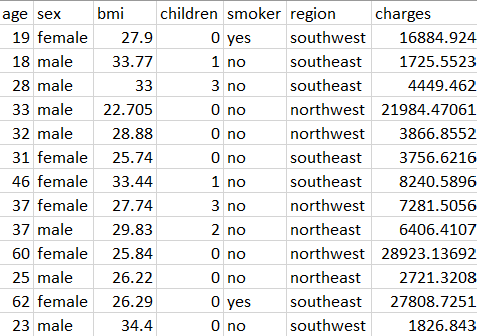
\includegraphics[height=6cm]{slide2}
	\end{center}
\end{spacing}
\end{frame}

\begin{frame}
	\begin{spacing}{1}
	\frametitle{Introduction and Motivation}
	\textbf{How to solve the above Problem ?}\\\pause
	\begin{itemize}
		\item Data Analysis\\\pause
		\item Cleaning the data and preparing the dataset for training\\\pause
		\item Make a model that best fits the data\\ \pause
		 	\begin{itemize}
		 		\item Maximum Likelihood Estimation(MLE)\\
		 		\item Maximum a Posterior Estimation(MAP)\\
		 		\item Bayesian Linear Regression(BLR)\pause
		 	\end{itemize}
	 	\item Make Predictions
	\end{itemize}
	\end{spacing}
\end{frame}

\section{Literature Survey}
\begin{frame}
	\begin{spacing}{1}
		\frametitle{Literature Survey}
		Consider the following graph:\\
		\begin{center}
			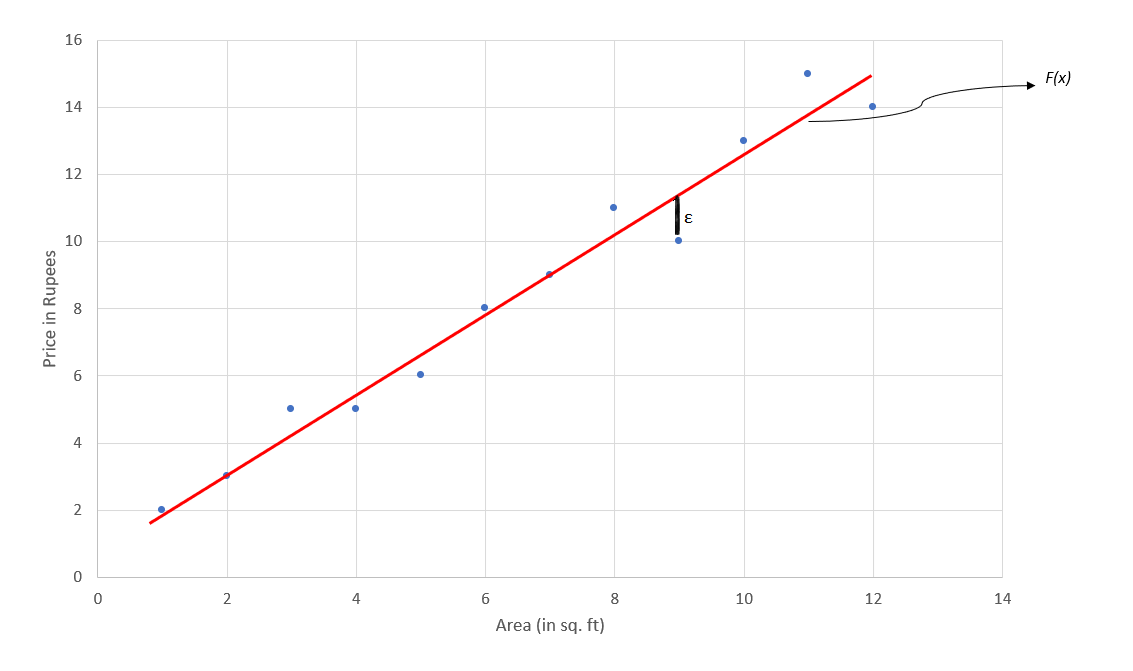
\includegraphics[width=12cm, height=4.5cm]{graph2}
		\end{center}\pause
		\begin{equation*}
			f(x)=\theta_{0} + \theta_{1}x
		\end{equation*}\pause
	\begin{equation*}
		y_{n}= f(x_{n}) + \epsilon, 
	\end{equation*}
	\hspace{4cm}where $\epsilon$ is the measurement noise.\pause
	\begin{equation*}
		\epsilon \sim \mathcal{N}(0,\sigma^2)
	\end{equation*}
	\end{spacing}
\end{frame}

\begin{frame}
	\begin{spacing}{1}
		\frametitle{Literature Survey}
		\framesubtitle{Problem Formulation}
		Let us consider the likelihood function
		\begin{equation*}
			p(y|x)= \mathcal{N}(y|f(x),\sigma^2)
		\end{equation*}
		where $x \in \mathbb{R}^D$ are the inputs,\\
		and $y \in \mathbb{R}$ are the targets.\\
		Here $D$ refers to the number of features.\\ 
		Also, $y= f(x) + \epsilon$ \\
		where $\epsilon \sim \mathcal{N}(0,\sigma^2)$ is an independent and identically distibuted random variable that represents the noise.\\\vspace{0.2cm}\pause
		\begin{equation*}
			f(x)=x^T\theta
		\end{equation*}
		where $x$ is the feature vector,\\
		and $\theta$ is the model parameters vector.\\ \vspace{0.2cm} \pause
		Hence,
		\begin{align*}
			p(y|x)&= \mathcal{N}(y|x^T\theta,\sigma^2)\\
			\Leftrightarrow y &= x^T\theta + \epsilon, \epsilon \sim \mathcal{N}(0,\sigma^2)
		\end{align*} 	
	\end{spacing}
\end{frame}

\begin{frame}
	\begin{spacing}{1}
		\frametitle{Literature Survey}
		\framesubtitle{Parameter Estimation}
		Consider the training set,
		\begin{equation*}
			Z=\{(x_{1},y_{1}), (x_{2},y_{2}), \dots, (x_{n},y_{n})\}
		\end{equation*}
		consisting of $N$ inputs $x_{n} \in \mathbb{R}^D$ and targets $y_{n} \in \mathbb{R}$, n=1, 2, \dots, N.\\ \pause \vspace{0.2cm}
		Now, $p(Y|X,\theta) = p(y_{1}, y_{2},\dots, y_{n}|x_{1}, x_{2}, \dots, x_{n}, \theta)$\\
		As we know that $y_{i}$ and $y_{j}$ are conditionally independent given their respective inputs $x_{i}$ and $x_{j}$.\\
		\begin{align*}
			\therefore p(Y|X,\theta)&=\prod_{n=1}^{N} p(y_{n}|x_{n}, \theta)\\
			&=\prod_{n=1}^{N} \mathcal{N}(y_n|x_n^T\theta,\sigma^2)
		\end{align*}
		where $X = \{x_{1}, x_{2}, \dots, x_{n}\}$ is the input set.\\
		and $Y = \{y_{1}, y_{2}, \dots, y_{n}\}$ is the target set.\\ 
	\end{spacing}
\end{frame}

\begin{frame}
		\begin{spacing}{1}
		\frametitle{Literature Survey}
		\framesubtitle{Maximum Likelihood Estimation}
		Maximizing the likelihood means maximizing the predictive distribution of the training data given the model parameters.\\
		Mathematically, we have to evaluate\\
		\begin{equation*}
			\theta_{ML} = \underset{\theta}{\arg\max}  P(Y|X,\theta)
		\end{equation*} \pause \vspace{0.2cm}
		\textbf{The negative log likelihood is also called Loss function.}\\
		\begin{align*}
			\mathcal{L}(\theta) &= \frac{\sum_{n=1}^{N}(y_{n}-x_{n}^T\theta)^2}{2\sigma^2}\\ 
			&=\frac{(y-X\theta)^T(y-X\theta)}{2\sigma^2} 
		\end{align*}
	\end{spacing}
\end{frame}

\begin{frame}
	\begin{spacing}{1}
		\frametitle{Literature Survey}
		\framesubtitle{Maximum Likelihood Estimation}
		\begin{align*}
			\boxed{\theta_{ML} = (X^TX)^{-1}X^Ty }
		\end{align*}
		where, 
		\begin{align*}
			X=\begin{bmatrix}
				x_{1}^{(1)} & x_{1}^{(2)} & \dots & x_{1}^{(D)}\\
				x_{2}^{(1)} & x_{2}^{(2)} & \dots & x_{2}^{(D)}\\
				. & . & .& .\\
				. & . & .& .\\
				. & . & .& .\\
				x_{N}^{(1)} & x_{N}^{(2)} & \dots & x_{N}^{(D)}
			\end{bmatrix} \in \mathbb{R^{NXD}}
		\end{align*}
		is the feature matrix consisting of $N$ training inputs and $D$ features.\\
		$y = \begin{bmatrix}
			y_{1}\\
			y_{2}\\
			.\\
			.\\
			.\\
			y_{n}
		\end{bmatrix} \in \mathbb{R}^N$ \hspace{2cm} and \hspace{2cm}
		$\theta = \begin{bmatrix}
			\theta_{1}\\
			\theta_{2}\\
			.\\
			.\\
			.\\
			\theta_{D}
		\end{bmatrix} \in \mathbb{R}^D$\\
	\end{spacing}
\end{frame}

\begin{frame}
	\begin{spacing}{1}
		\frametitle{Literature Survey}
		\framesubtitle{Maximum Likelihood Estimation}
		Consider the following graph:\\
		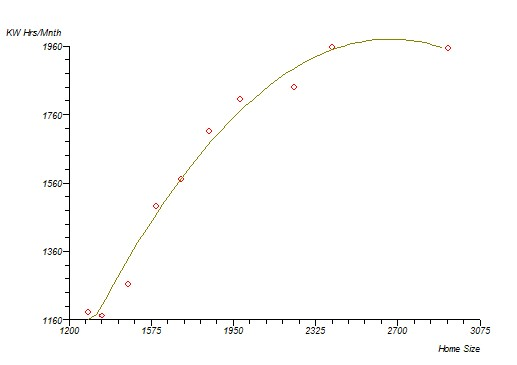
\includegraphics[height=7cm]{graph4}\\ 
	\end{spacing}
\end{frame}

\begin{frame}
	\begin{spacing}{1}
		\frametitle{Literature Survey}
		\framesubtitle{Maximum Likelihood Estimation}
		%\begin{align*}
		$p(y|x,\theta) = \mathcal{N}(y|\phi^T(x)\theta, \sigma^2)$\\
		$\Leftrightarrow y = \phi^T(x)\theta + \epsilon = \sum_{k=0}^{K-1}\theta_{k}\phi_{k}(x) +\epsilon$
		%\end{align*}
		where $\phi$ : $\mathbb{R}^D \rightarrow \mathbb{R}^K$ is a non linear transformation of inputs $x$.\\
		$\phi_{k}$ : $\mathbb{R}^D \rightarrow \mathbb{R}$ is the $k$th component of the vector $\phi$.\\
		\pause For example\\
		\begin{tiny}
			\begin{equation*}
				\phi(x) = \begin{bmatrix}
					1\\ x\\ x^2\\ .\\ .\\ .\\ x^{K-1}
				\end{bmatrix}
				= \begin{bmatrix}
					\phi_{0}(x)\\ \phi_{1}(x)\\ \phi_{2}(x)\\ .\\ .\\ .\\ \phi_{K-1}(x)
				\end{bmatrix} \in \mathbb{R}^K
			\end{equation*}
		\end{tiny}\pause
	\begin{equation*}
		\boxed{\theta_{ML} = (\Phi^T\Phi)^{-1}\Phi^Ty}  
	\end{equation*}
	\end{spacing}
\end{frame}

\begin{frame}
	\begin{spacing}{1}
		\frametitle{Literature Survey}
		\framesubtitle{Overfitting In Linear Regression}
		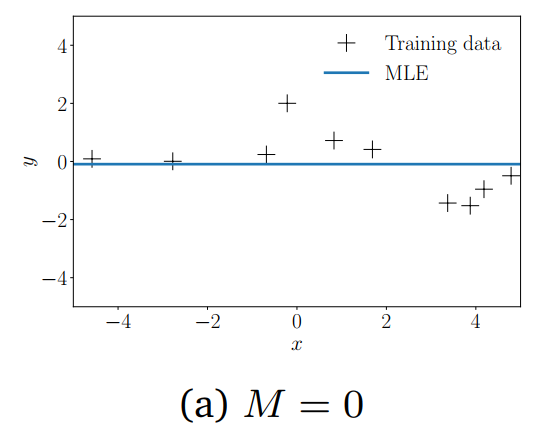
\includegraphics[width=3.8cm, height=5cm]{graph5} 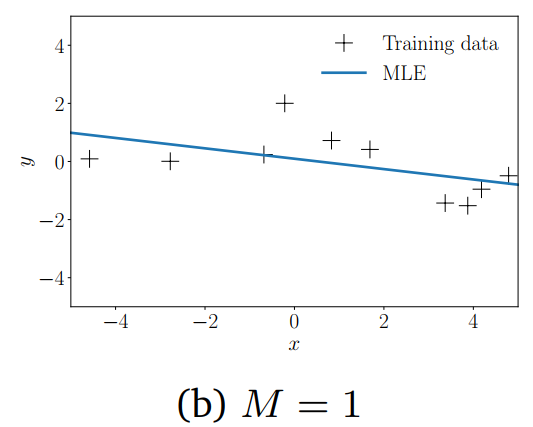
\includegraphics[width=3.8cm,height=5cm]{graph6} 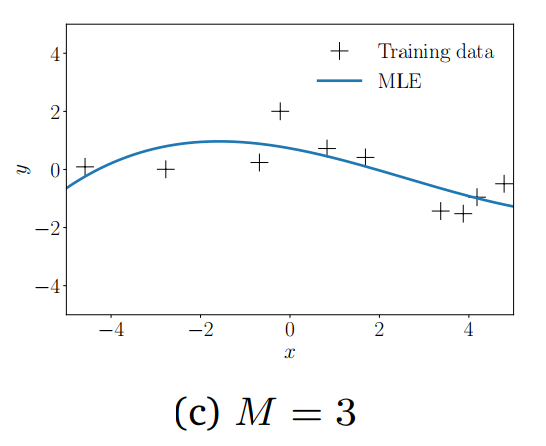
\includegraphics[width=3.8cm,height=5cm]{graph7}\\
		
	\end{spacing}
\end{frame}

\begin{frame}
	\begin{spacing}{1}
		\frametitle{Literature Survey}
		\framesubtitle{Overfitting In Linear Regression}
		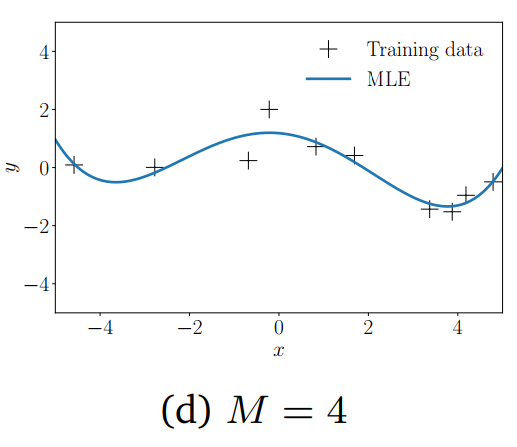
\includegraphics[width=3.8cm, height=5cm]{graph8} 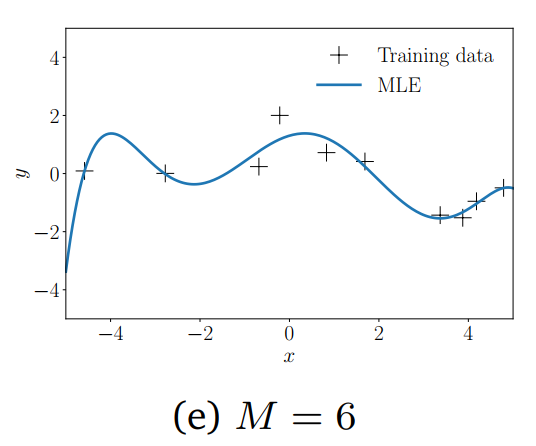
\includegraphics[width=3.8cm, height=5cm]{graph9} 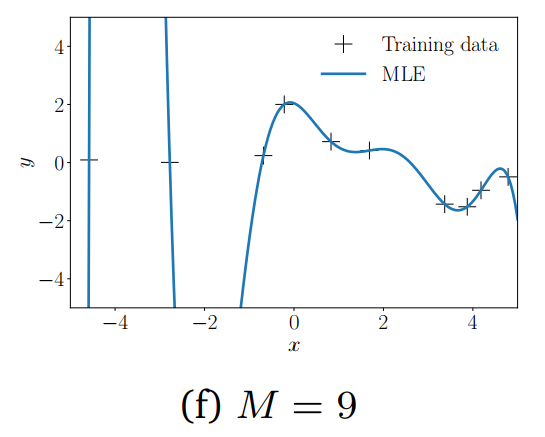
\includegraphics[width=3.8cm, height=5cm]{graph10}\\
		
	\end{spacing}
\end{frame}
		
\begin{frame}
	\begin{spacing}{1}
		\frametitle{Literature Survey}
		\framesubtitle{Overfitting In Linear Regression}
		\begin{center}
			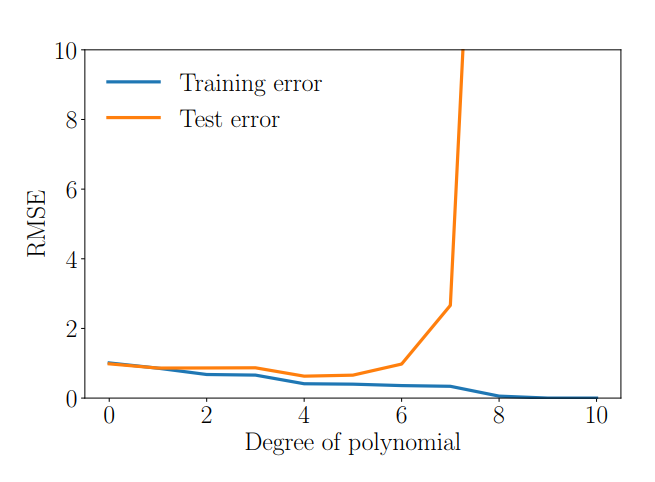
\includegraphics[height=8cm]{graph11}\\
		\end{center}
		
	\end{spacing}
\end{frame}

\begin{frame}{Literature Survey}
	\begin{spacing}{1}
		\framesubtitle{Maximum a Posterior(MAP) Estimation}
		\textbf{Why overfitting occurs? How to overcome it?}\pause
		\begin{align*}
			p(\theta) &= \mathcal{N}(0, 1)
		\end{align*}
		\begin{center}
			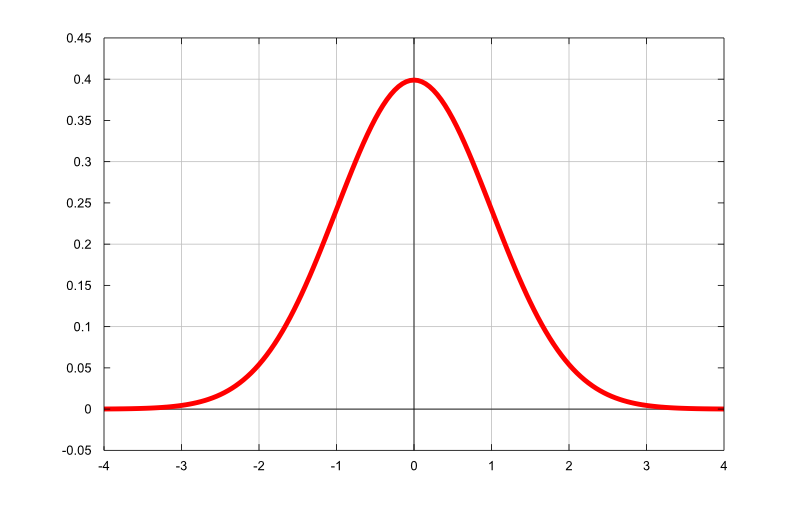
\includegraphics[width=\columnwidth, height=4.5cm]{graph12}
		\end{center}\pause
		\textbf{Given our training data $X, Y$. Here we will maximize the posterior distribution $p(\theta|X, Y)$. This method is called maximum a posterior(MAP) estimation.}\\
	\end{spacing}
\end{frame}

\begin{frame}{Literature Survey}
	\begin{spacing}{1}
		\framesubtitle{Maximum a Posterior(MAP) Estimation}
		Now applying Baye's theorum -
		\begin{equation*}
			p(\theta|X, Y) = \frac{p(Y|X, \theta)p(\theta)}{p(Y|X)}
		\end{equation*}\pause
		\begin{equation*}
			\log p(\theta|X, Y) =  \log p(Y|X, \theta) + \log p(\theta) + const 
		\end{equation*}\pause
		We assume that $p(\theta) = \mathcal{N}(0, b^2I)$.\\ \pause
		\begin{align*}
			\boxed{\theta_{MAP} = (\Phi^T\Phi + \frac{\sigma^2}{b^2}I)^{-1}\Phi^Ty}
		\end{align*}\pause
		\begin{equation*}
			\theta_{RLS} = (\Phi^T\Phi + \lambda I)^{-1}\Phi^Ty
		\end{equation*} 
		
	\end{spacing}
\end{frame}

\begin{frame}{Literature Survey}
	\begin{spacing}{1}
		\framesubtitle{Maximum a Posterior(MAP) Estimation}
		
		\begin{center}
			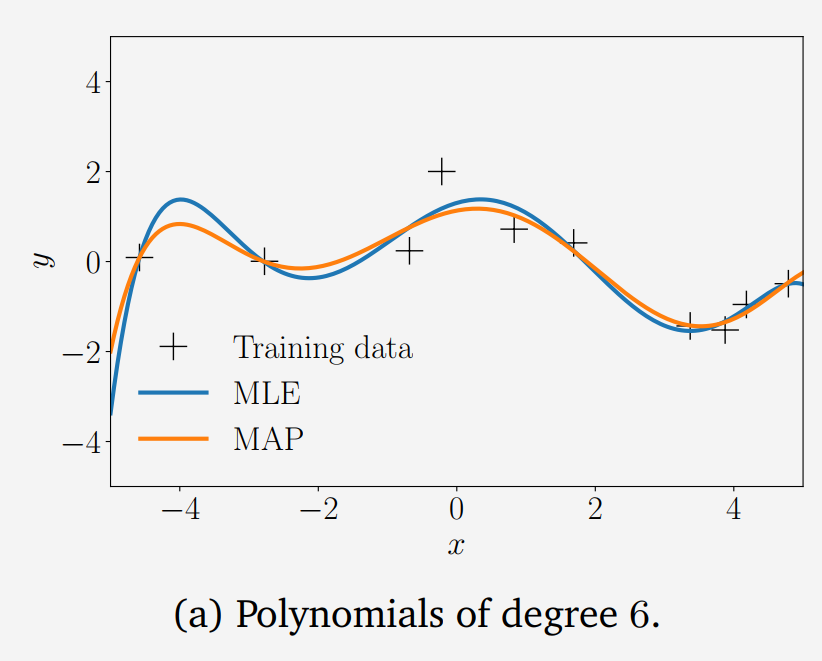
\includegraphics[height=5cm,width=4.8cm]{garph13} 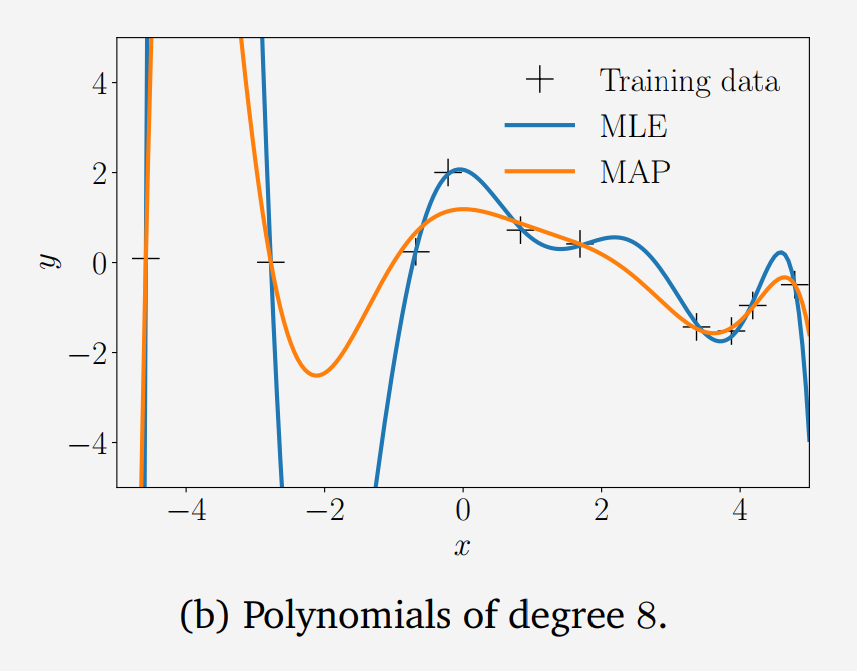
\includegraphics[height=5cm,width=4.8cm]{graph14} \\
		\end{center}
				
	\end{spacing}
\end{frame}
		

\begin{frame}{Literature Survey}
	\begin{spacing}{1}
		\framesubtitle{Bayesian Linear Regression}
		
		Bayesian linear regression does not attempt to compute a point estimate of the parameters, but instead the full posterior distribution over parameters($\theta$) is taken into account when making predictions. This means we compute the mean over all plausible parameter settings.\\\pause
		For Bayesian linear regression, consider,\\
		\textbf{prior} $p(\theta) = \mathcal{N}(m_o, S_o)$\\
		\textbf{likelihood} $p(y|x, \theta) = \mathcal{N}(y|\phi^T(x)\theta, \sigma^2)$\\\pause
		\vspace{0.2cm}
		\textbf{Prior Predictions}
		\begin{align*}
			p(y_*|x_*) &= \int p(y_*|x_*, \theta)p(\theta)d\theta\\
			&= E_\theta[p(y_*|x_*, \theta)]
		\end{align*}\pause
		\begin{equation*}
			p(y_*|x_*) = \mathcal{N}(\phi^T(x_*)m_o, \phi^T(x_*)S_o\phi(x_*) + \sigma^2)
		\end{equation*}\pause
		But if we want to find out the distribution of $f(x_*) = \phi^T(x)\theta$.
		\begin{equation*}
			f(x_*) = \mathcal{N}(\phi^T(x_*)m_o, \phi^T(x_*)S_o\phi(x_*))
		\end{equation*}
	\end{spacing}
\end{frame}

\begin{frame}{Literature Survey}
	\begin{spacing}{1}
		\framesubtitle{Bayesian Linear Regression}
		\textbf{Example} If we chose parameter prior to be $p(\theta) = \mathcal{N}(0, \frac{I}{4})$.
		\begin{center}
			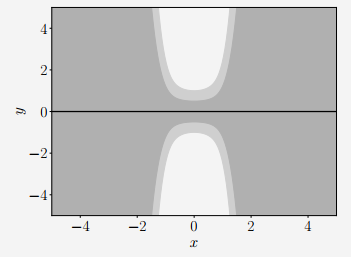
\includegraphics[height=5.5cm, width=5cm]{graph15}
			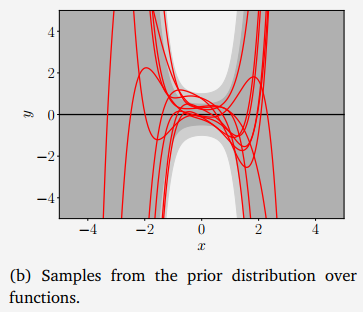
\includegraphics[height=5.5cm, width=5cm]{graph16}
		\end{center}
\end{spacing}
\end{frame}


\begin{frame}{Literature Survey}
	\begin{spacing}{1}
		\framesubtitle{Bayesian Linear Regression}
		\textbf{Posterior Predictions}\\
		\begin{footnotesize}
		\begin{equation*}
			p(\theta|X, Y) = \frac{p(Y|X, \theta)p(\theta)}{p(Y|X)}
		\end{equation*}\pause
	\begin{align*}
		p(\theta|X, Y) &= \mathcal{N}(\theta|m_N, S_N)\\
		S_N &= (\sigma^{-2}\Phi^T\Phi + S_o^{-1})^{-1}\\
		m_N &= S_N(\sigma^{-2}\Phi^Ty + S_o^{-1}m_o)
	\end{align*}\pause
		\begin{align*}
			p(y_*| X, Y, x_*) &= \int p(y_*|x_*, \theta)p(\theta|X, Y)d\theta\\
			&= \int \mathcal{N}(y_*|\phi^T(x_*)\theta, \sigma^2)\mathcal{N}(\theta|m_N, S_N)d\theta\\
			&= \mathcal{N}(y_*| \phi^T(x_*)m_N, \phi^T(x_*)S_N\phi(x_*) + \sigma^2)
		\end{align*}\pause

		\begin{equation*}
			\therefore f(x_*) = \mathcal{N}(\phi^T(x_*)m_N, \phi^T(x_*)S_N\phi(x_*))
		\end{equation*}
	
	\end{footnotesize}
	\end{spacing}
\end{frame}

\begin{frame}{Literature Survey}
	\begin{spacing}{1}
		\begin{center}
			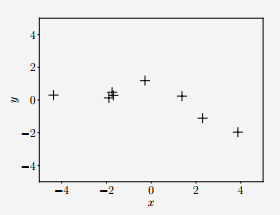
\includegraphics[height=6cm, width=5.5cm]{graph17}
			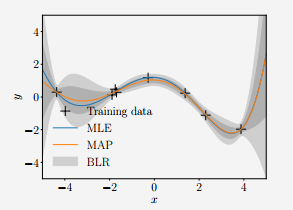
\includegraphics[height=6cm, width=5cm]{graph18}
		\end{center}
		\end{spacing}
\end{frame}

\section{Main Results}
\begin{frame}{Main Results}
	\begin{spacing}{1}
		Given dataset,
		\begin{center}
			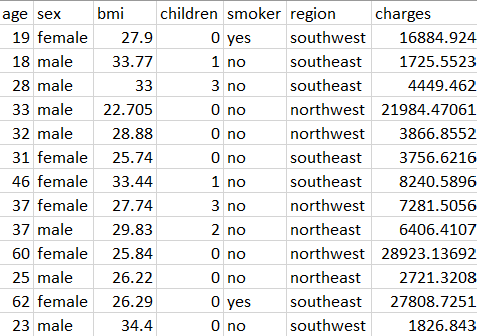
\includegraphics[height=5cm, width=8cm]{slide2}
		\end{center}
		
	\end{spacing}
\end{frame}

\begin{frame}{Main Results}
	\begin{spacing}{1}
		\begin{center}
			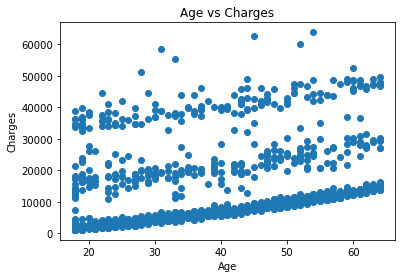
\includegraphics[height=5.5cm,width=8cm]{work2}\\
		\end{center}
		\hspace{3.75cm}{Correlation between Age and Charges = 0.2999}
	\end{spacing}
\end{frame}

\begin{frame}{Main Results}
	\begin{spacing}{1}
		\begin{center}
			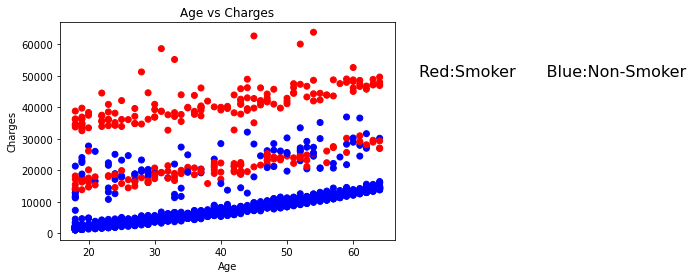
\includegraphics[height=6cm,width=11cm]{work4}
		\end{center}
	\end{spacing}
\end{frame}
\begin{frame}{Main Results}
\begin{spacing}{1}
	\textbf{Smokers}
	\begin{center}
		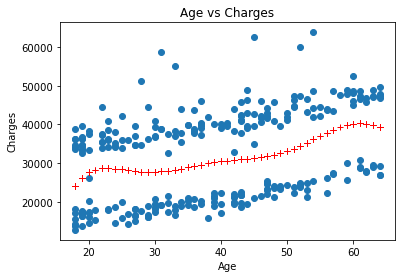
\includegraphics[height=6cm, width=8cm]{work6}
	\end{center}
\end{spacing}
\end{frame}

\begin{frame}{Main Results}
	\begin{spacing}{1}
		\textbf{Smokers with BMI>30}
		\begin{center}
			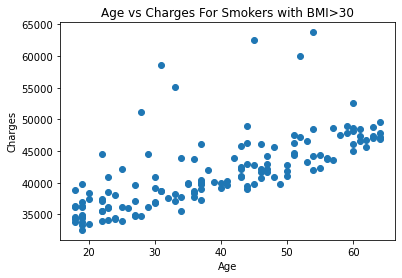
\includegraphics[height=6cm, width=8cm]{work7}
		\end{center}
	\end{spacing}
\end{frame}

\begin{frame}{Main Results}
	\begin{spacing}{1}
		\textbf{Smokers with BMI>30}
		\begin{center}
			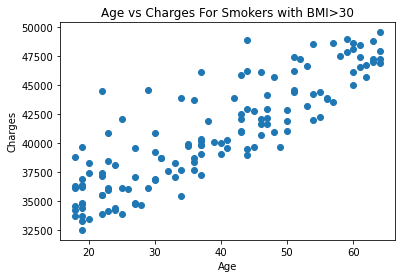
\includegraphics[height=5.5cm, width=8cm]{work8}
		\end{center}
	\hspace{3.5cm}{Correlation between Age and Charges = 0.8623745}
	\end{spacing}
\end{frame}

\begin{frame}{Main Results}
	\begin{spacing}{1}
		\textbf{Smokers with BMI>30}
		\begin{center}
			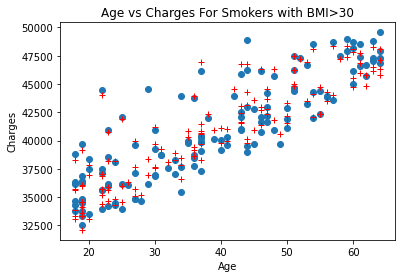
\includegraphics[height=6cm, width=8cm]{work10}
		\end{center}
	\end{spacing}
\end{frame}

\begin{frame}{Main Results}
	\begin{spacing}{1}
		\textbf{Smokers with BMI<=30}
		\begin{center}
			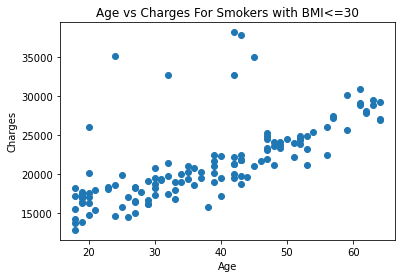
\includegraphics[height=6cm, width=8cm]{work11}
		\end{center}
	\end{spacing}
\end{frame}

\begin{frame}{Main Results}
	\begin{spacing}{1}
		\textbf{Smokers with BMI<=30}
		\begin{center}
			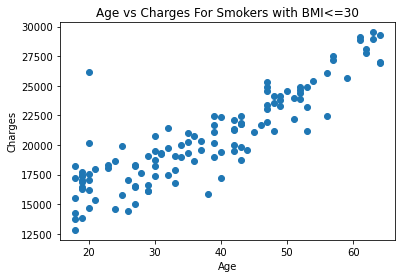
\includegraphics[height=5.5cm, width=8cm]{work12}
		\end{center}
	\hspace{3.5cm}{Correlation between Age and Charges = 0.8623745}
	\end{spacing}
\end{frame}

\begin{frame}{Main Results}
	\begin{spacing}{1}
		\textbf{Smokers with BMI<=30}
		\begin{center}
			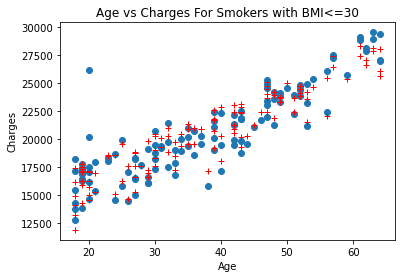
\includegraphics[height=6cm, width=8cm]{work14}
		\end{center}
	\end{spacing}
\end{frame}

\begin{frame}{Main Results}
	\begin{spacing}{1}
		\textbf{Non- Smokers}
		\begin{center}
			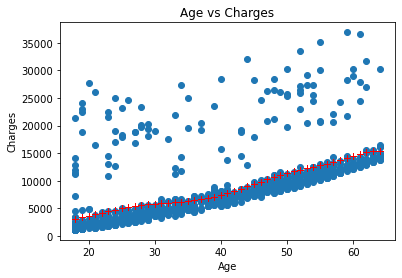
\includegraphics[height=6cm, width=8cm]{work16}
		\end{center}
	\end{spacing}
\end{frame}

\begin{frame}{Main Results}
	\begin{spacing}{1}
		\textbf{Non- Smokers}
		\begin{center}
			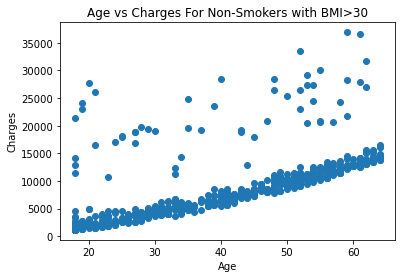
\includegraphics[height=6cm, width=5.4cm]{work17}
			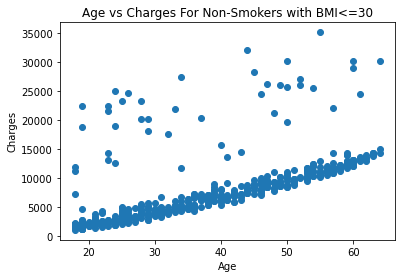
\includegraphics[height=6cm, width=5.4cm]{work18}
		\end{center}
	\end{spacing}
\end{frame}

\begin{frame}{Main Results}
	\begin{spacing}{1}
		\textbf{Non- Smokers}
		\begin{center}
			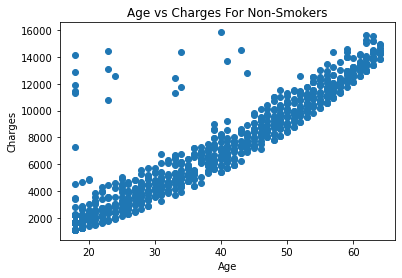
\includegraphics[height=5.5cm, width=8cm]{work19}
		\end{center}
	\hspace{3.5cm}{Correlation between Age and Charges = 0.92874}
	\end{spacing}
\end{frame}

\begin{frame}{Main Results}
	\begin{spacing}{1}
		\textbf{Non- Smokers}
		\begin{center}
			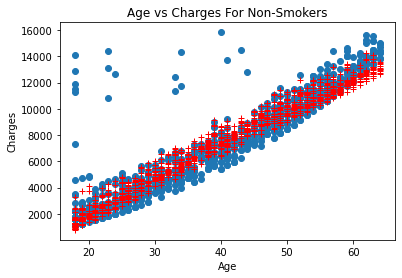
\includegraphics[height=6cm, width=8cm]{work21}
		\end{center}
	\end{spacing}
\end{frame}

\begin{frame}{Main Results}
	\begin{spacing}{1}
		\begin{center}
			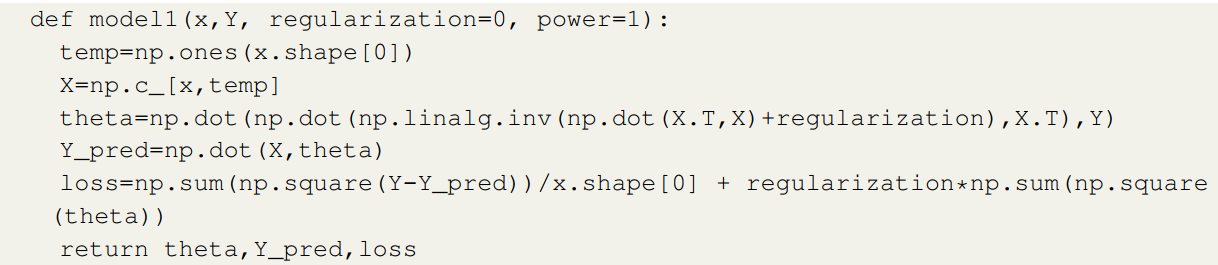
\includegraphics[height=4.5cm, width=11cm]{model}
		\end{center}
	\end{spacing}
\end{frame}

\begin{frame}{Main Results}
	\begin{spacing}{1}
		\begin{center}
			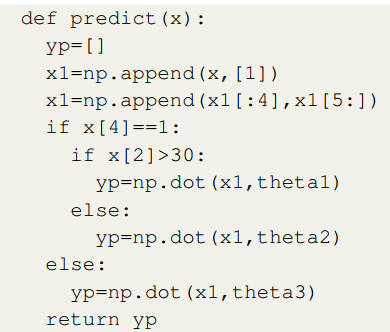
\includegraphics[height=6cm, width=6cm]{predict}
		\end{center}
	\end{spacing}
\end{frame}

\section{Conclusion}
\begin{frame}{Conclusion}
	\begin{spacing}{1}
		\begin{itemize}
			\item 	Based on the understandings and results from the Literature Survey we trained a model that predicts the insurance price for a person given his Age, Sex, BMI, Number of Children, Smoking Status and Region. \pause
			\item First we analysed the dataset. The given data was too much scattered to be able to get a good model that fits it. So we segregated the data for smokers and non-smokers separately. Then we further segregated it using BMI. Still some scattered points were left due to unknown reasons of a particular person so we made a upper-bound to the data. This way we trained the model and finally we were able to get a decent result.
		\end{itemize}
	\end{spacing}
\end{frame}

\section{References}
\begin{frame}{References}
	\begin{spacing}{1}
		\begin{thebibliography}{99}
			\bibitem{B} Marc Peter Deisenroth, A. Aldo Faisal, Cheng Soon Ong - Mathematics For Machine Learning-Cambridge University Press (2019)
			\bibitem{B} https://www.coursera.org/learn/machine-learning/home/welcome
			\bibitem{C}https://towardsdatascience.com/
	\end{thebibliography}
	\end{spacing}
\end{frame}

\begin{frame}
	\begin{block}{}
		\begin{center}
			\textcolor{brown}{\textbf{\em \huge  THANK YOU}}
		\end{center}
	\end{block}
\end{frame}
\end{document}